% =====================================================================
% Snippet: confusion-matrix.tex
% =====================================================================
% USAGE: N×N confusion matrix with cell values and diagonal emphasis.
% Used for classification result panels.
%
% Copy %% COPY-START / END, replace:
%   - matrix data: \def\cmdata{...} 16 values for 4x4 (row-major)
%   - class_names: \def\classnames{...}
%   - cell_size, origin
% =====================================================================

\documentclass[tikz,border=10pt]{standalone}
\usepackage{xcolor,tikz}
\usetikzlibrary{positioning,calc}

\definecolor{acaBlueLine}{HTML}{3060A8}
\definecolor{cmLo}{HTML}{F0F4FB}
\definecolor{cmHi}{HTML}{3060A8}
\definecolor{acaGreyLine}{HTML}{606060}

\begin{document}
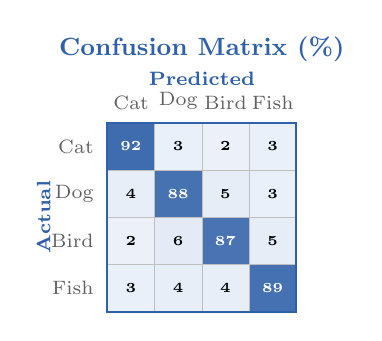
\begin{tikzpicture}

%% COPY-START =========================================================

% --- DATA: 4x4 row-major (true class i predicted as class j) ---
% Diagonal should be high (correct predictions)
\def\cmdata{%
  92, 3, 2, 3,%      Cat row
  4, 88, 5, 3,%      Dog row
  2, 6, 87, 5,%      Bird row
  3, 4, 4, 89%       Fish row
}
\def\classnames{Cat, Dog, Bird, Fish}
\def\xO{0}
\def\yO{0}
\def\cs{0.6}        % cell size
\def\N{4}

% --- HEADER: predicted column labels (top) ---
\foreach [count=\j] \cname in \classnames {
  \pgfmathsetmacro\cx{\xO + (\j - 0.5) * \cs}
  \node[anchor=south, font=\scriptsize, color=acaGreyLine]
    at (\cx, \yO + 0.05) {\cname};
}

% --- HEADER: actual row labels (left) ---
\foreach [count=\i] \cname in \classnames {
  \pgfmathsetmacro\cy{\yO - (\i - 0.5) * \cs}
  \node[anchor=east, font=\scriptsize, color=acaGreyLine]
    at (\xO - 0.05, \cy) {\cname};
}

% --- CELL FILL + VALUES ---
\foreach [count=\idx] \val in \cmdata {
  \pgfmathtruncatemacro\rowI{int((\idx - 1) / \N) + 1}
  \pgfmathtruncatemacro\colJ{int(mod(\idx - 1, \N)) + 1}
  \pgfmathsetmacro\cx{\xO + (\colJ - 0.5) * \cs}
  \pgfmathsetmacro\cy{\yO - (\rowI - 0.5) * \cs}
  % intensity by value
  \fill[cmHi!\val!cmLo]
    (\cx - \cs/2, \cy - \cs/2) rectangle (\cx + \cs/2, \cy + \cs/2);
  % text contrast: white on dark, dark on light
  \pgfmathsetmacro\textc{ifthenelse(\val > 50, "white", "black")}
  \edef\textcA{\textc}
  \node[anchor=center, font=\tiny\bfseries]
    at (\cx, \cy) {\textcolor{\textcA}{\val}};
}

% --- GRID + BORDER ---
\draw[step=\cs cm, acaGreyLine!40, line width=0.2pt]
  (\xO, \yO) grid (\xO + \N * \cs, \yO - \N * \cs);
\draw[acaBlueLine, line width=0.7pt]
  (\xO, \yO) rectangle (\xO + \N * \cs, \yO - \N * \cs);

% --- AXIS LABELS ---
\node[anchor=south, font=\scriptsize\bfseries, color=acaBlueLine]
  at (\xO + \N * \cs / 2, \yO + 0.35) {Predicted};
\node[anchor=south, font=\scriptsize\bfseries, color=acaBlueLine, rotate=90]
  at (\xO - 0.6, \yO - \N * \cs / 2) {Actual};

% --- TITLE ---
\node[anchor=south, font=\small\bfseries, color=acaBlueLine]
  at (\xO + \N * \cs / 2, \yO + 0.65) {Confusion Matrix (\%)};

%% COPY-END ===========================================================

\end{tikzpicture}
\end{document}
